\documentclass{natureprintstyle}
%\documentclass{nature}
\bibliographystyle{naturemag}
\usepackage{epsfig,caption}
\usepackage{color}
\usepackage{bm}
\usepackage{graphicx}
\usepackage{longtable}
\usepackage{amssymb}
\usepackage{rotating}
\usepackage{latexsym}
\usepackage{hyperref}
\usepackage{float}
\usepackage{soul}

%\usepackage[switch]{lineno}
%\linenumbers

%%%%%%%%%%%%%%%%%%%%%%%%%%%%%%%%%%%%%%%%%%%%%%%%%%%%%%%%%%%%%%%%%%%
% comment for selecting the best figures to go on web for:
%@arxiver{jvds_sami_vsigma_ellip_LOESS_Age_paper.pdf,jvds_sami_vsigma_ellip_LOESS_Age_transform_paper_resubmit.pdf} 
%%%%%%%%%%%%%%%%%%%%%%%%%%%%%%%%%%%%%%%%%%%%%%%%%%%%%%%%%%%%%%%%%%%

%journal commands
\newcommand{\apj}{Astrophys. J.}
\newcommand{\spie}{Proc. SPIE}
\newcommand{\pasp}{Publ. Astron. Soc. Pac.}
\newcommand{\apjs}{Astrophys. J. Supp.}
\newcommand{\araa}{Annu. Rev. Astron. Astrophys.}
\newcommand{\mnras}{Mon. Not. R. Astron. Soc.}
\newcommand{\apjl}{Astrophys. J. Let.}
\newcommand{\aap}{Astron. Astrophys.}
\newcommand{\aj}{Astron. J.}
\newcommand{\nat}{Nature}
\newcommand{\na}{New Astron. Rev.}
\newcommand{\aaps}{A\&AS}
\newcommand{\procspie}{Proc. SPIE}

%%%%%%%%%%%%%%%%%%%%%%%%%%%%%%%%%%%%%%%%%%%%%%%%%%%%%%%%%%%%%%%%%%%
% my commands

\newcommand{\lcdm}{$\Lambda$CDM}
\newcommand{\hst}{{\it HST}}
\newcommand{\efr}{$R_{\mathrm{eff}}$}
\newcommand{\galfit}{{\sc Galfit}}
\newcommand{\mbh}{$\mathcal M_{\rm BH}$}
\newcommand{\lhost}{$L_{\rm host}$}
\newcommand{\mr}{$Mag_{\rm ~R}$}
\newcommand{\jcap}{Journal of Cosmology and Astroparticle Physics}
\newcommand{\halpha}{${\it H}\alpha$}
\newcommand{\hbeta}{${\it H}\beta$}
\newcommand{\sersic}{S\'ersic}
\newcommand{\lenstronomy}{{\sc Lenstronomy}}
\newcommand{\reff}{{$R_{\mathrm{eff}}$}}
%\newcommand{\kms}{km~s$^{\rm -1}$}
\newcommand{\kms}{\ifmmode{\,\rm{km}\, \rm{s}^{-1}}\else{$\,$km$\,$s$^{-1}$}\fi}
\newcommand{\sigstar}{{$\sigma_*$}}
\newcommand{\mstar}{{$M_*$}}
\newcommand{\Mgii}{Mg$_{\rm II}$}
\newcommand{\Civ}{C$_{\rm IV}$}
\newcommand{\farcs}{\mbox{\ensuremath{.\!\!^{\prime\prime}}}}% fractional arcsecond symbol: 0.''0
\newcommand{\sam}{\texttt{SAM}}
\newcommand{\mbii}{\texttt{MBII}}

%%%%%%%%%%%%%%%%%%%%%%%%%%%%%%%%%%%%%%%%%%%%%%%%%%%%%%%%%%%%%%%%%%%

\newcommand{\ding}[1]{\textcolor{red}{[{\bf Xuheng}: #1]}} 
\newcommand{\aklant}[1]{\textcolor{blue}{[{\bf AKB}: #1]}} 

\newcommand{\red}[1]{{ \textcolor{red}{#1}}}
\newcommand{\blue}[1]{{ \textcolor{blue}{#1}}}

\title{
%From predictions to observation: scaling relations between supermassive black holes and their host galaxies at $1< z<2$
A successful observational test of black hole and galaxy co-evolution models since $z\sim1.7$
%The first comparison between the observation and simulation of the scaling relations between supermassive black holes and their host galaxies at $1.2< z<1.7$
}
\author{Xuheng Ding$^{1,2}$, 
Tommaso Treu$^{1}$, 
John D. Silverman$^{3, 4}$,
Aklant K. Bhowmick$^{5,6}$,
N. Menci$^{7}$,
Tiziana Di Matteo$^{5}$
}

\begin{document}

\maketitle

\let\thefootnote\relax\footnote{
\begin{affiliations}
\item {Department of Physics and Astronomy, University of California, Los Angeles, CA, 90095-1547, USA} 
\item {School of Physics and Technology, Wuhan University, Wuhan 430072, China}
\item {Kavli Institute for the Physics and Mathematics of the Universe (WPI), The University of Tokyo, Kashiwa, Chiba 277-8583, Japan}
\item {Department of Astronomy, School of Science, The University of Tokyo, 7-3-1 Hongo, Bunkyo, Tokyo 113-0033, Japan}
\item{McWilliams Center for Cosmology, Dept. of Physics, Carnegie Mellon University, Pittsburgh PA 15213, USA}
\item{Department of Physics, University of Florida, Gainesville, FL 32611, USA}
\item{INAF Osservatorio Astronomico di Roma, via Frascati 33, I-00078 Monteporzio, Italy}
\end{affiliations}
}

\begin{abstract}
Supermassive black holes (SMBHs) ubiquitously occupy the center of massive galaxies in the local Universe and beyond. Their growth in mass (\mbh) appears to be closely linked to the physical properties of their host galaxies\cite{Mag++98, F+M00, M+H03, H+R04, Gul++09}, in particular the relation between \mbh ~and stellar mass (\mstar). With the origin of this correlation far from being fully understood, simulations have been a promising means to further interpret the observations over the last eight billion years ($z\lesssim1$) thus enabling substantial progress in this field. Constraints at higher redshifts ($z>1$), when most of the SMBHs acquired their mass, are more sensitive to initial conditions and the growth mechanisms and thus may be able to identify inaccurate or missing physics in the models. For this purpose, we have constructed a unique sample of 32 actively-accreting SMBHs at $1.2 < z < 1.7$ ($\sim 8.5-10$ billion years ago) with accurate BH and stellar masses with the latter based on multi-band \hst\ imaging. We directly compare the measurements with two independent state-of-the-art projects, the hydrodynamic simulation \texttt{MassiveBlackII} (\mbii) and the semi-analytic model (\sam).  After applying the observational selection function to models to account for bias, we find that both \mbii\ and \sam\ agree well with the data, in terms of the central distribution. However, accounting for observational errors, the dispersion in the mass ratio between \mbh\ and \mstar\ is significantly more consistent with the \mbii\ prediction ($\sim0.3$~dex), than with the \sam\ ($\sim0.7$~dex) one. Hence, our observations can distinguish between the different recipes adopted in the models. The mass relations in \mbii ~are highly dependent on AGN feedback while the relations in the \sam\ are more sensitive to galaxy merger events triggering nuclear activity. Moreover, the intrinsic scatter in the mass ratio of our high-$z$ sample is comparable to that observed in the local sample, all but ruling out the proposed scenario the correlations are purely stochastic in nature arising from some sort of cosmic central limit theorem. Our results support the hypothesis of AGN feedback being responsible for a causal link between the SMBH and its host galaxy, resulting in a tight correlation between their respective masses.

\end{abstract}

%\section{Introduction}

Various models have been proposed to explain the connection between SMBH and their host galaxies. A possible physical link may be feedback from an Active Galactic Nucleus (AGN) phase, assuming that a fraction of the AGN energy is injected into their surrounding gas thus regulating the growth of the SMBH and its host galaxy. In this scenario, AGN activity heats and unbinds a significant fraction of the gas and inhibits star formation. An alternatively and more indirect connection is one where AGN accretion and star formation are fed through a common gas supply~\cite{Cen2015, Menci2016}. A completely different view holds that the statistical convergence from galaxy assembly alone (i.e., dry mergers) may reproduce the observed correlations without any direct physical mechanisms~\cite{Peng2007, Jahnke2011, Hirschmann2010}. From this central limit theorem, a stochastic cloud at high-$z$ (higher dispersion) would end up with scaling relations as observed today with lower dispersion.

To understand this connection, recent works~\cite{Park15, Tre++07, Bennert11, Woo++08} have measured the scaling relations out to intermediate redshift {($0.3\lesssim z \lesssim1$)} by studying AGN and their host galaxies with {\it Hubble Space Telescope} ({\it HST}) and found an `observed' evolution in which the growth of SMBHs predates their host galaxies. However, the observational evidence of such evolution at higher-$z$ is under debate since it depends on our understanding of systematic uncertainties and selection effects~\cite{Tre++07,Lauer2007}. Therefore, an improper consideration of the uncertainties and selection effects may lead to an {\it apparent} evolution and result in an overestimate of the significance of the evolution\cite{Volonteri2011}.

%Why comparison between data and model.
%Summary of recently works.
%The reason to extend to high redshift.
Simulations are effective at helping to understand this connection and rule out theories and assumptions that could not be definitively verified by observations alone. In particular, simulations can be used to quantify the impact of systematic uncertainties and selection biases with observational data. Recent studies, based on several simulations, show agreement with the observational data at intermediate redshifts ($z\lesssim1$). For example, the state-of-the-art cosmological hydrodynamical simulation of structure formation (\texttt{MassiveBlackII}) has been utilized to compare the predicted scaling relations to \hst\ observation at $0.3<z<1$ that show a positive evolution where the SMBH growth predates that of its the host galaxy~\cite{DeG++15}. Several other works have investigated scaling relations using large-volume simulations, resulting in good agreement with the local relation and some redshift evolution, including the Magneticum Pathfinder SPH Simulations~\cite{Steinborn2015}, the Evolution and Assembly of GaLaxies and their Environments (EAGLE) suite of SPH simulations~\cite{Schaye2015}, and Illustris moving mesh simulation\cite{Sijacki2015, Vogelsberger2014, Li2019}. Besides hydrodynamic simulations, semi-analytic models~\cite{Menci2014, Menci2016} have also made remarkable progress and recovered the local scaling relations~\cite{Kormendy13}. However, comparisons between simulations and the observed scaling relations, based on high-resolution \hst\ imaging, are still mostly limited to $z<1$ due to prior limitations of observational data.

% The work that we want to do
	%Sample selection
	%The advantage of our measurements
	%Compare to which simulation? (some introduction)
	%Any expectation?
	%mention the scatter.
To push our knowledge of the mass relations to earlier epochs, we have been analyzing a sample of 32 \hst-observed AGN systems over the redshift range $1.2<z<1.7$ from three deep survey fields, namely COSMOS~\cite{Civano2016}, (E)-CDFS-S~\cite{Lehmer2005, Xue2011}, and SXDS~\cite{Ueda2008} (D19~\cite{Ding2019} hereafter). The redshift range of our targets is chosen to be high enough ($z>1$) to establish the mass ratios of accreting SMBHs and to make direct comparisons to the models, while low enough ($z<2$) to limit the effect of surface brightness dimming that would lower the success rate of detecting the underlying host galaxy. 
We selected our AGN sample in a well-defined window based on the \mbh\ and Eddington ratio, as shown in Figure~1 in D19. As shown in that Figure, the \mbh\ are well below the knee of the BH mass distribution to avoid strong selection bias. In addition, the Eddington ratios are mostly above $0.1$ to ensure homogeneity.

We measure reliable \mbh\ and host properties (i.e., \mstar) with a quantitative assessment of systematic effects. Specifically, \mbh\ is determined using published near-infrared spectroscopic observations of the broad \halpha\ emission line, which eliminates potential systematic uncertainties that may arise from switching to Balmer lines in the local universe to the \Mgii\ or \Civ\ UV lines for distant galaxies. Regarding the detection of the host galaxies, the X-ray selected nature of the sample results in slightly lower nuclear-to-host ratios, which facilitates the inference of the host light. We employ \hst/WFC3 to obtain high-resolution (0\farcs0642 per pixel) imaging data and adopt a state-of-the-art technique to perform a 2-D flux profile decomposition to measure the light of the host galaxy. Moreover, 21/23 systems have \hst/ACS imaging data, which enables us to assess the colors of the host, hence the rest frame R-band magnitude (\mr) and stellar mass (\mstar) (see METHODS and the descriptions in D19). 
%We furthermore combining them with the ground-based photometry to carry out the SED fitting, and thus derive the reliable host rest-frame R band luminosity and stellar mass.

%\begin{figure}[t]
%\includegraphics[width=0.9\linewidth]{AGN_selection.pdf}
%\caption{The selection for the 32 AGN sample. The top and right panels are the BH mass function and Eddington ratio function. \ding{More descriptions are needed if Figure1 is finally decided to show.}
%}
%\label{fig:AGN_select}
%\end{figure}

To compare with simulations, we use two independent efforts, the \texttt{MassiveBlackII} (\texttt{MBII})~\cite{Khandai2015} and the semi-analytic model (\texttt{SAM})~\cite{Menci2014}. These simulations are based on independent model strategies, i.e., hydrodynamic simulation for \mbii\ and semi-analytic model for \sam, respectively. The \mbii\ simulation is the highest resolution at the size of a comoving volume $V_{\rm box} = (100~{\rm Mpc}~h^{-1})$, including a self-consistent model for star formation, black hole accretion, and associated feedback. The large simulation volume enables the model galaxies and SMBHs to evolve independently; the large dynamic range in mass and high spatial resolution meet the requirements to investigate their individual galaxies. While high-resolution N-body simulations can study specific galaxy systems, an understanding of the physical mechanisms influencing the scaling relations require an analytical description of such processes to be implemented into existing semi-analytic models including the \sam. In previous works, \mbii~\cite{Huang2018, DeG++15, Khandai2015,Bhowmick2019} and \sam~\cite{Menci2014, Menci2016} have made high successful predictions; we refer the interested readers to the METHODS section for more details.

We note that the absolute determination of stellar mass carries significant uncertainty, both observationally and theoretically. Depending on definitions of stellar mass, on the assumed initial mass function, and possibly on the implementation of star formation in the models, the absolute value of \mstar\ (hence the absolute normalization, i.e., \mbh/\mstar) can vary by up to a factor of two. In contrast, the scatter around the mean correlation is a relative quantity, which is less affected by this uncertainty. Thus, in this work, we mainly focus on the scatter as a diagnostic tool, even though in the future more information could be extracted by this kind of comparison if the %absolute stellar mass could be constrained more accurately in the simulations.}
better measures~(i.e., more consistent with techniques for determining observed \mstar) of stellar masses can be defined for the simulated galaxies.

%\section*{Results}
%Selection effect into account
Using \mbii, we identify a sample of simulated AGNs at $z=1.5$ (see METHOD) and compare their predicted scaling relations to the observed ones. We take the measurement uncertainty and selection biases into account to ensure a fair comparison. First, we inject random noise to the simulated sample to mimic the scatter in our data due to measurement errors, i.e., $\Delta$\mbh $=0.4$~dex, $\Delta$\mr$=0.3$~dex, $\Delta$\mstar$=0.17$~dex, and $\Delta L_{\rm bol}=0.03$~dex, respectively. We then select the sample that falls into the same targeting window to match the observed sample (Figure~\ref{fig:selectfunc}). 

In Figure~\ref{fig:MM_comp} (left panel), we compare the relation \mbh--\mstar~between observations and the \mbii\ simulation. First, it is clear that the simulated and observed samples are in good agreement. To quantify the agreement level, we perform a linear regression to fit the simulated relations and estimate the best-fit inference. To make a direct comparison, we fix the same slope value and obtain the best-fit intercept value for the observation. We find that the \mbh-\mstar\ relations are in agreement within the relatively large scatter of the sample. Furthermore, we compare the scatter by calculating the standard derivation of the residuals of the linear regression. We find that the simulations and the observations have the same amount of scatter $0.25-0.3$~dex (see METHODS).

\begin{figure}[t]
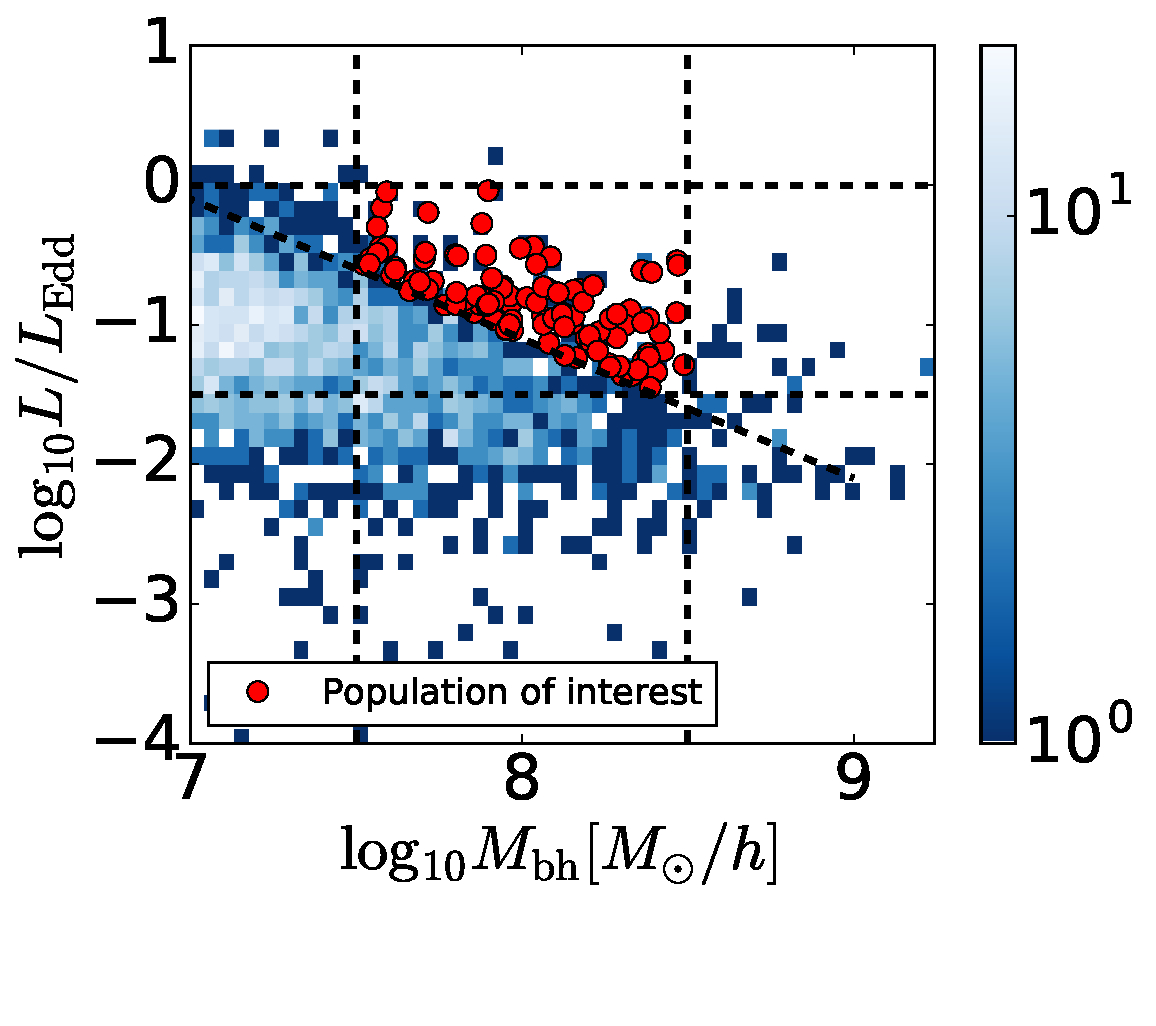
\includegraphics[width=1.2\linewidth]{MBII_selectfunc.pdf}
\caption{The same selection window as adopted for selecting the \mbii\ simulated sample. The brown background cloud shows the simulated number density of the overall \mbii\ sample at $z=1.5$. We add the random uncertainty to the simulation and select the ones fall into the targeting region (i.e., blue colored). The orange dots are the \hst\ observed sample.}
\label{fig:selectfunc}
\end{figure}
%comparison to simulation (flux ratio also)

\begin{figure*}[t]%[!b]
\begin{tabular}{c c}
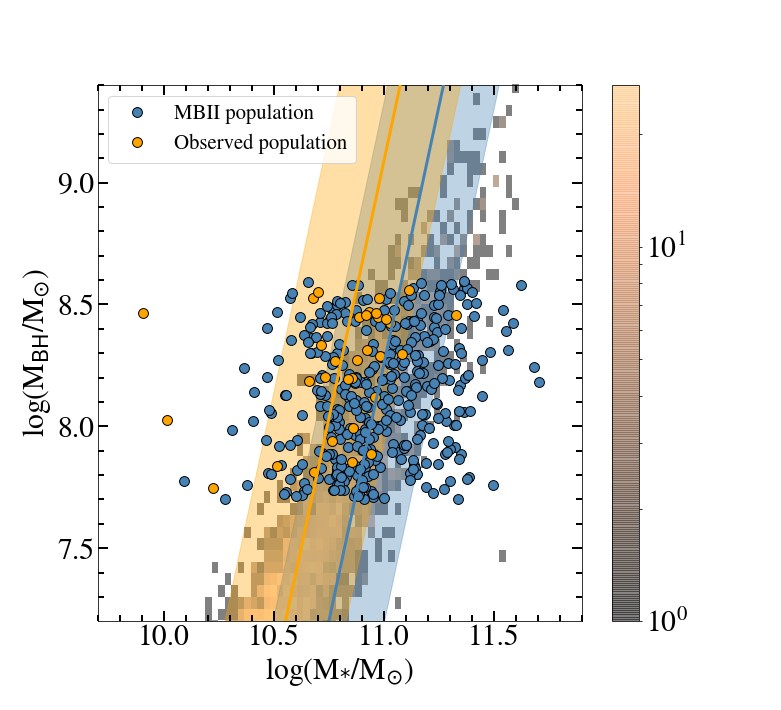
\includegraphics[trim = 0mm 0mm 65mm 0mm, clip, width=0.47\linewidth]{MBII_MM.pdf} &
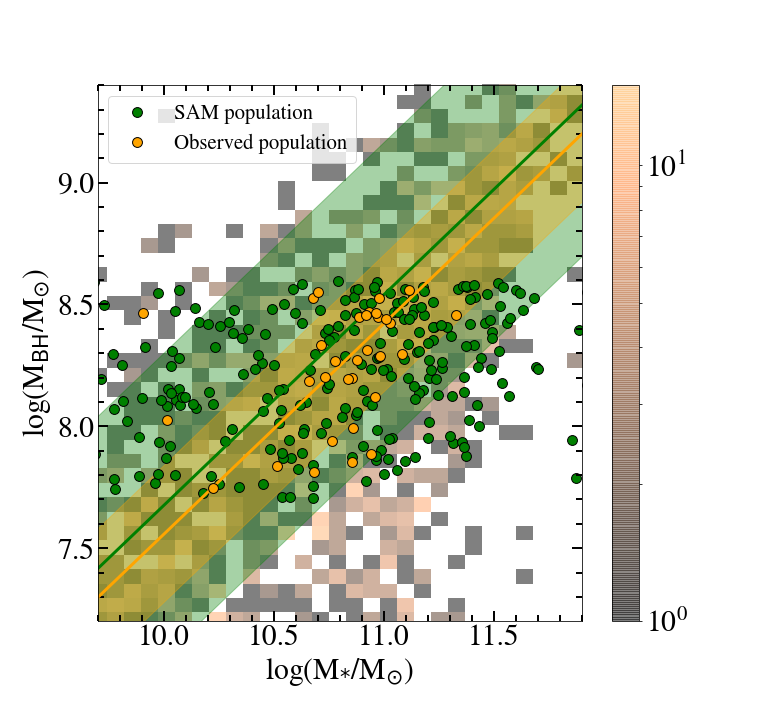
\includegraphics[trim = 0mm 0mm 65mm 0mm, clip, width=0.47\linewidth]{SAM_MM_consider_nois.pdf} \\
\end{tabular}
\caption{(Left) Comparison of the observed (orange dots) and simulated (blue dots) \mbh--\mstar\ relation. The blue line is the best-fit result for the \mbii\ sample, with the colored region indicating the standard derivation of the residual. By fixing the slope to match the simulated data, the orange color shows the result for the observed data set. The grey cells in the background show the full \mbii\ simulated SMBHs. (Right) The equivalent plot is displayed for the \sam\ sample (green color) in the right panel.}
\label{fig:MM_comp}
\end{figure*}

We also compare our data to the predictions by the \sam\ model. Rather than N-body simulation which produces individual simulating objects, the \sam\ model uses the density clouds to describe the possibility of the samples. 
%We consider the sample at $z=1.5$ epoch for two sample sets, including the overall sample and the selected sample, as shown in Figure~\ref{fig:SAM_comp}. We find that considering the selecting effect, the direct prediction by \sam\ is well matched to the observed relations.
%We do not estimate the scatter for \sam\ model, but visually see that the observed relations are mostly located on top of the hot cloud, showing that the observed scatter should not be larger than the model one. \ding{This is not right yet. But if consider the scatter in the same way, the \sam\ have large scatter?}
%Yet this is not a proper comparison since the direct sample from \sam\ does not include the scattering effect by the measurement uncertainty.
To make a direct comparison, we first randomly generate an overall \sam\ sample based on the probability clouds at $z=1.5$. Then, as in the \mbii\ analysis, we inject random scatter in the sample to account for uncertainties and apply the observational selection function. The resulting comparison of the  \mbh-\mstar\ relation are shown in Figure~\ref{fig:MM_comp} (right panel). We find that the best-fit result by the \sam\ model is well matched to the observation. However, the scatter of the \sam\ model is significantly larger ($0.7$~dex) than observed (this is the total scatter accounting for the intrinsic scatter in the \sam\ distribution, observational uncertainties, and selection effects).  


%\begin{figure*}[t]%[!b]
%\begin{tabular}{c c}
%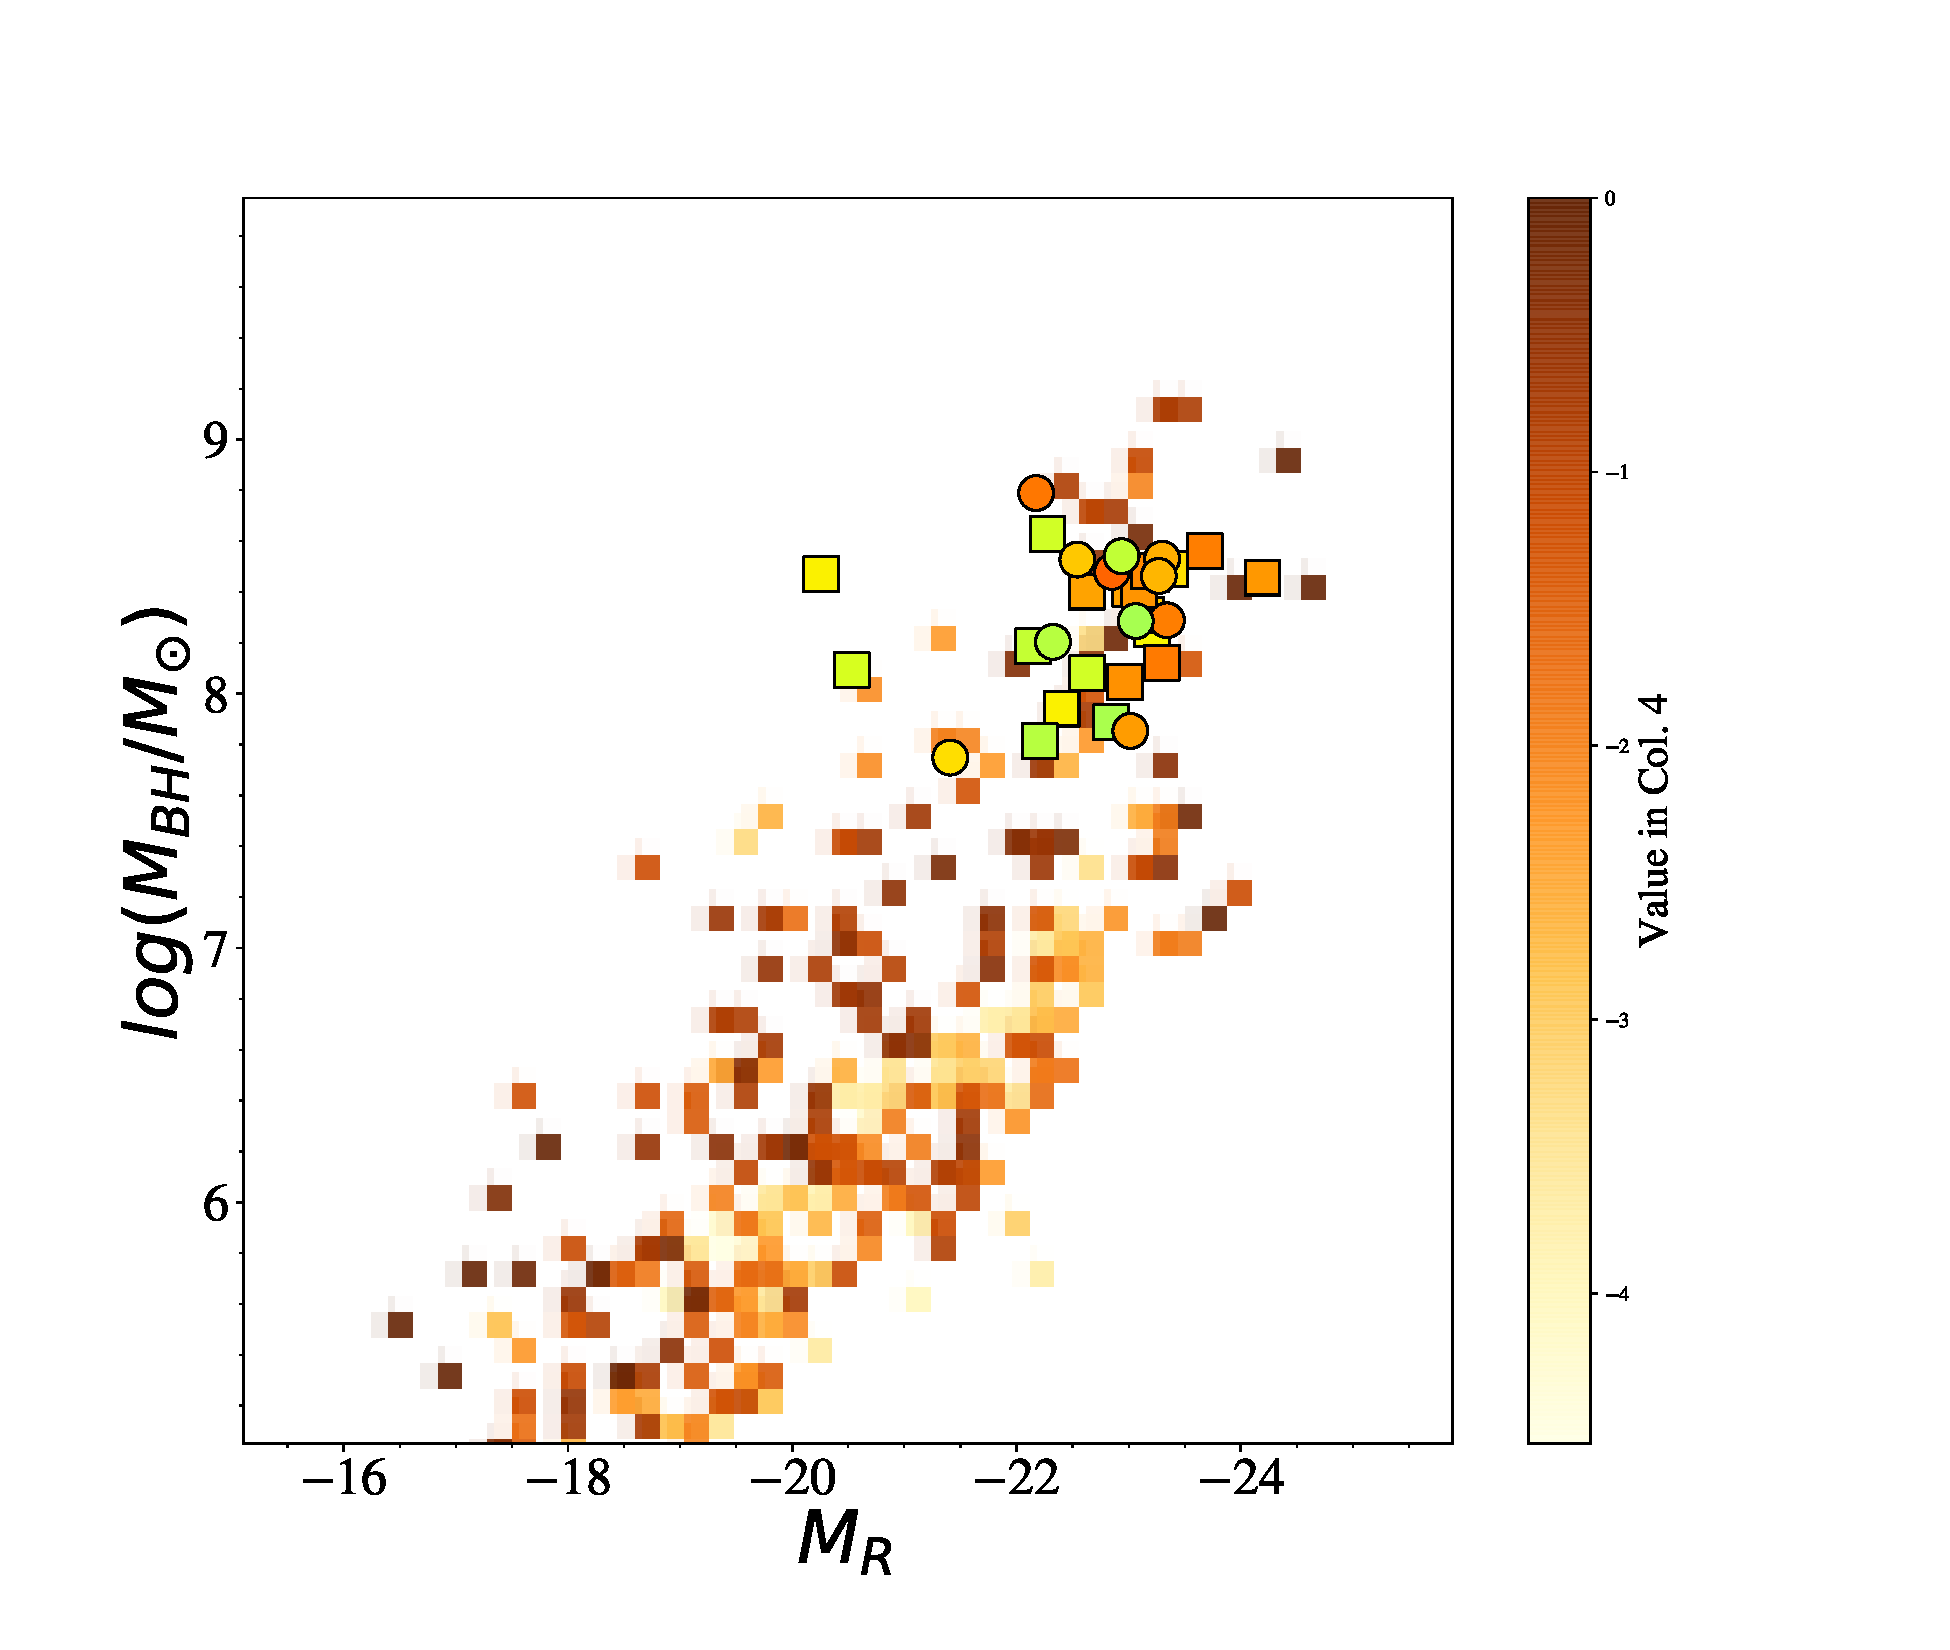
\includegraphics[trim = 0mm 0mm 24mm 0mm, clip, width=0.45\linewidth]{SAM_ML.pdf} &
%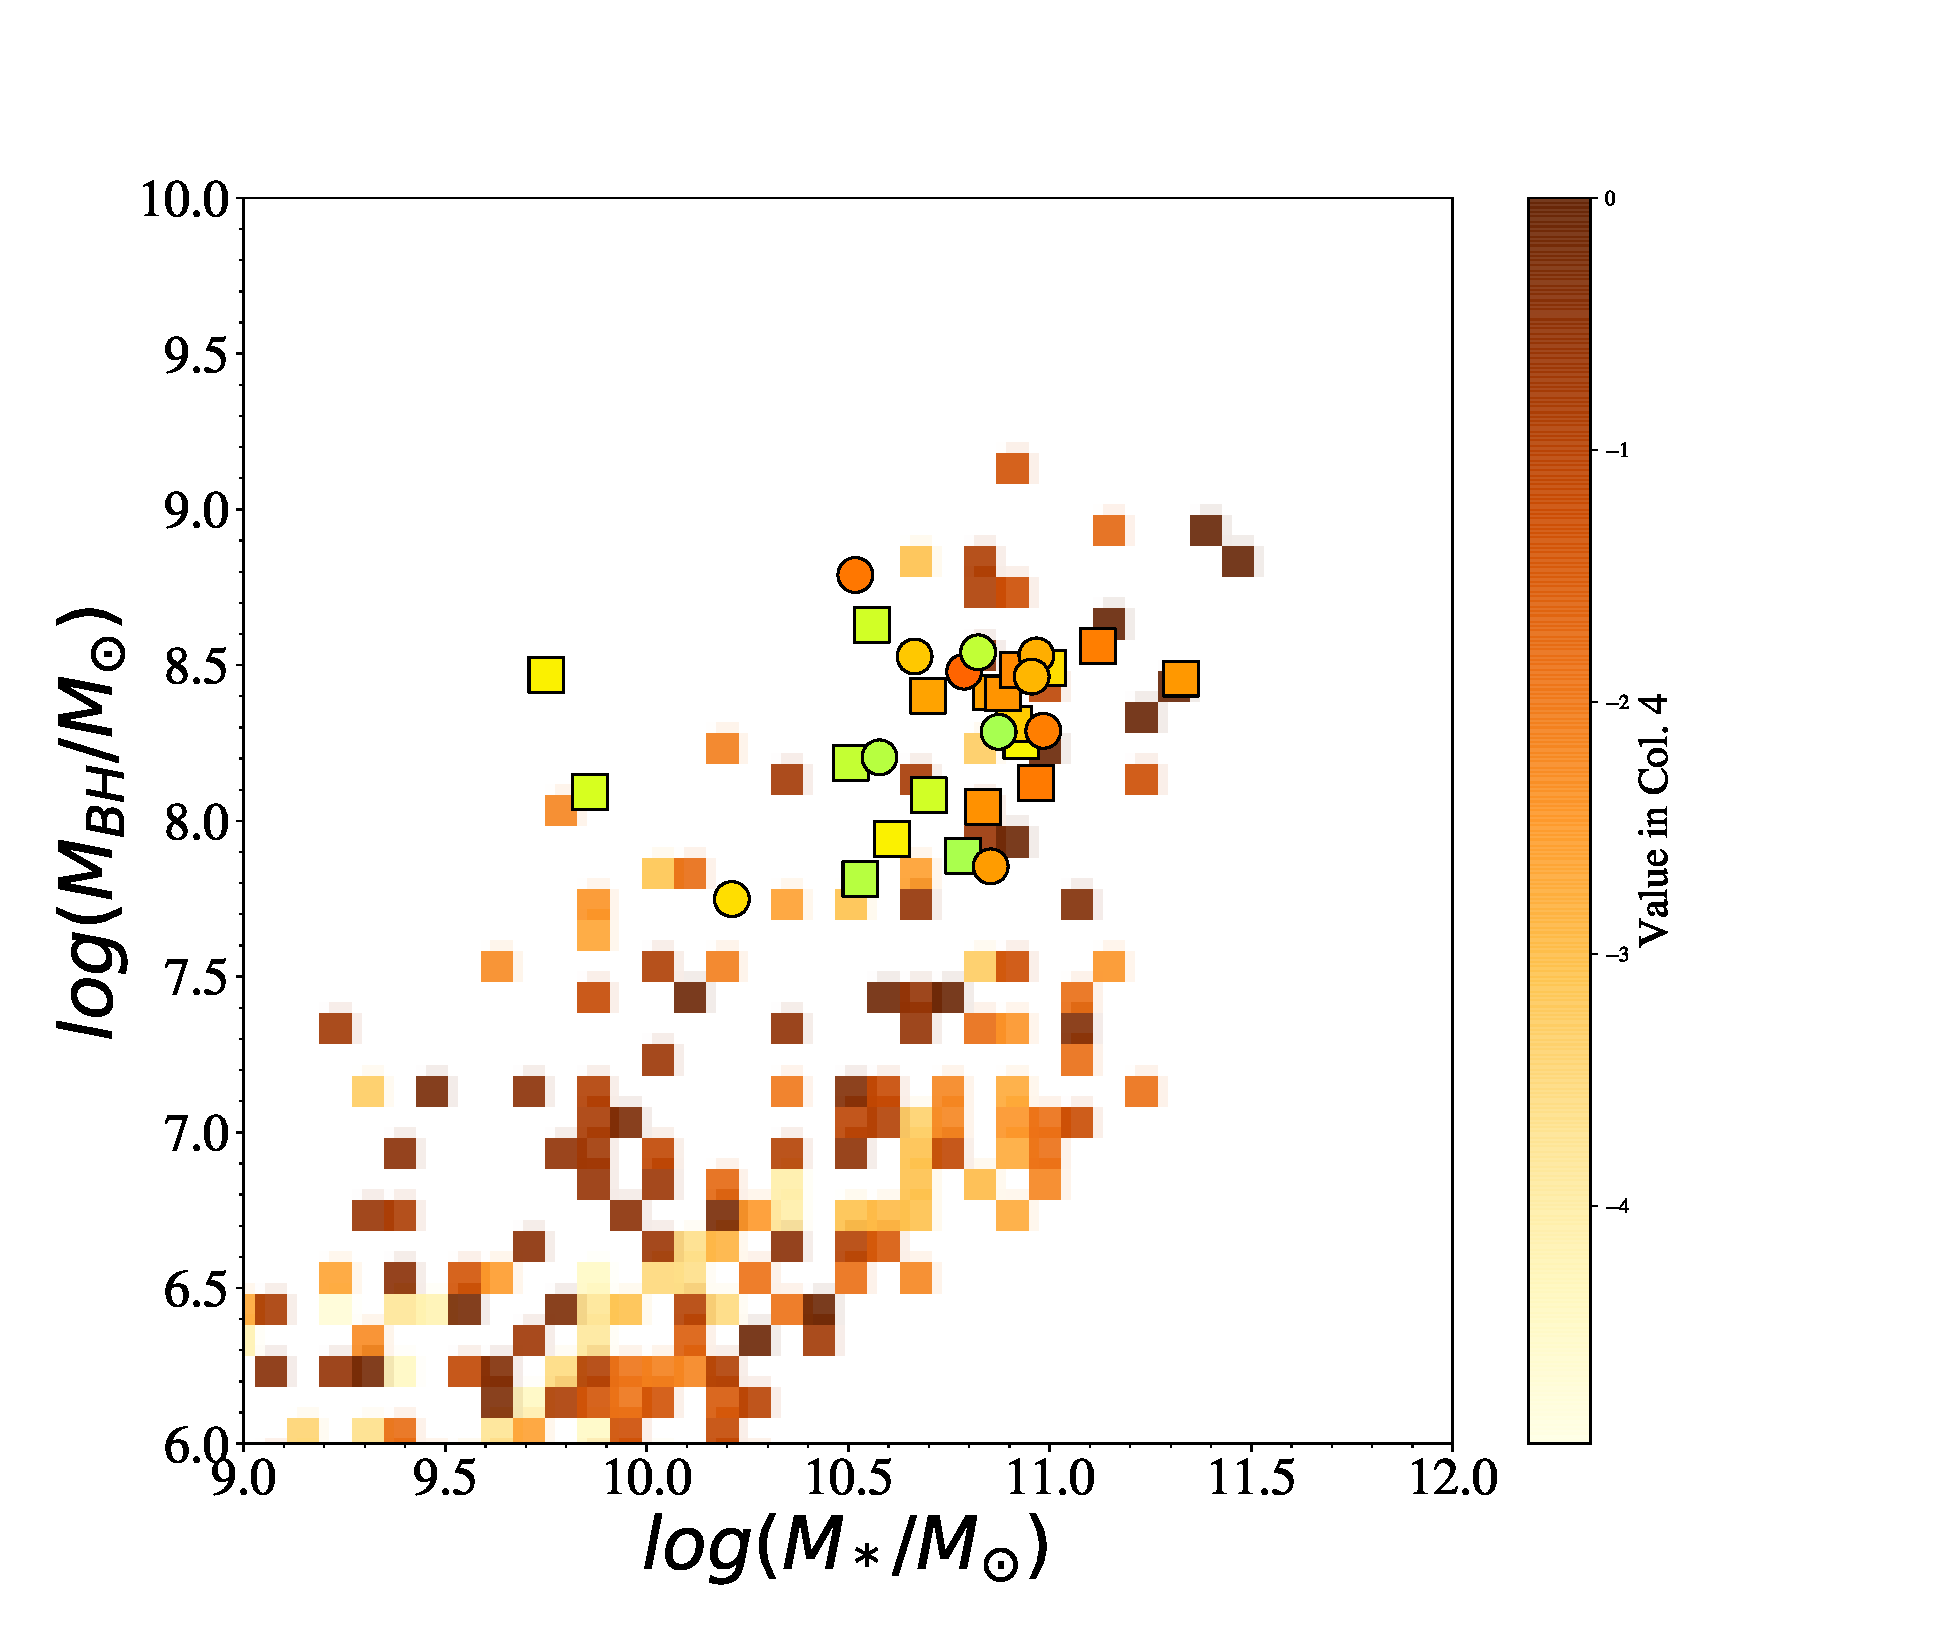
\includegraphics[trim = 30.5mm 0mm 0mm 0mm, clip, width=0.45\linewidth]{SAM_MMstar.pdf} \\
%\end{tabular}
%\caption{Similar to the Figure~\ref{fig:MM_comp}, but for a direct comparison to the observation using SAM's model. The blue background contours show the possibility distribution for the overall sample, and the red contours indicate the distributions after considering the selecting effect. We presented our observational data as yellow dots. Note that this comparison has not taken the measurement uncertainties into account yet. 
%}
%\label{fig:SAM_comp}
%\end{figure*}

To test if any unexpected selection effects exist, we compare the distribution of the host-total flux ratio among these three samples. For the observed sample, we calculate the flux ratio at the imaging band, i.e., \hst/WFC3. For the simulated sample, we consider the AGN bolometric correction~\cite{Elvis1994} to estimate the AGN light flux at WFC3/F125W band. We compare their host-total flux histogram distribution in Figure~\ref{fig:comp_hist} and see that the three samples are well matched to each other. The median values for the flux ratio distribution of the observed, \mbii, \sam\ sample are $37.3\%$, $32.3\%$, and $42.8\%$, respectively. We perform the Kolmogorov-Smirnov (KS) test the inferred p-values are $0.34$ (for observed -- \mbii) and $0.14$ (for observed -- \sam), respectively. This result indicates the three samples have similar host-to-total light ratio distribution.

\begin{figure}[t]
\includegraphics[width=0.9\linewidth]{comp_host_ratio.pdf}
\caption{Comparison of the host to total flux ratio distribution for the three referred samples, median value indicated. The observational selection function is applied to the simulated samples to allow for a fair comparison.
}
\label{fig:comp_hist}
\end{figure}

In terms of their central distribution, the \mbii\ simulation and \sam\ model are both in agreement with the observational data. However, the scatter distinguishes between the two models. The  the scatter in \mbii\ simulation is consistent to the observational one ($\sim0.3$~dex), while \sam\ sample has significantly larger scatter ($\sim0.7$~dex). Thus, the implementation of AGN feedback in \mbii\ passes our stringent observational test. The \sam\ model also consider the AGN feedback. However, in contrast to \mbii, the feeding process for the SMBH accretion is driven by the 2-body interaction of galaxy mergers, and thus may be more stochastic and lead to the larger scatter. More specifically, in the \sam\ model the encounters are assumed to trigger the feedback, and the fraction of gas that feeds the SMBH is related to the parameters of the  encounter, which introduces additional scatter since it depends on the properties of both interacting galaxies (see METHODS). As a result, the \sam\ cloud extends to the high \mbh\ with low stellar mass, which may not exist. The consistency between \mbii\ and observations provides important observational evidence in support of the hypothesis that there is a causal link (i.e., AGN feedback) between the evolution of SMBH and that of their host galaxies.

Without any physical mechanisms, it has been shown that just due to the the central limit theorem~\cite{Peng2007, Jahnke2011, Hirschmann2010} scaling relations may emerge from random mergers, starting from a stochastic cloud in the early universe. In this scenario, the scatter of the scaling relations has to increase with redshift. Our observations contradict this hypothesis. In fact, our inferred intrinsic scatter of the observed sample is $\sim0.25$~dex, which is no more than the typical scatter of local relations reported in the literature ($\sim0.35$~dex)~\cite{Kormendy13, Gul++09}. Of course, the intrinsic scatter of our high-$z$ sample could be inaccurate, since we use the \mbii\ overall sample as a proxy to estimate the level of intrinsic scatter for the real data, but it is unlikely that systematic errors would conspire to {\it reduce} scatter.
Also, the observed \mbh\ are estimated using the robust \halpha\ line, which could have lower uncertainties level than expected (i.e., $\Delta$\mbh$<0.4$~dex), resulting in an overestimating of the error-budget and thus underestimating of intrinsic scatter, but again it is hard to imagine that the \halpha\ \mbh\ estimators be much more precise than an factor of two. 

Extending this study to even higher redshift would be very beneficial, probing closer to the epoch of formation of massive galaxies and supermassive blackes. For higher redshift, the {\it James Webb Space Telescope} may provide high-quality imaging data of AGNs at redshift up to $z\sim7$. In the low redshift Universe, wide-area surveys with Subaru/HSC, LSST, and WFIRST offer much promise to build samples for studying these mass ratios and dependencies on other factors (e.g., environment).

%\textcolor{blue}{The details of the results could be presented.\\
%0. Compare the color of the sample?\\
%1. 2D KS test? \\
%2. More insightful inference from the comparing?
%}

%Discuss the result, What does this mean?

% \textcolor{blue}{If the final results show such feature:}
%The result also shows that the \mbh-\mstar\ relation has less scatter than the \mbh-\lhost\ relation, suggesting that the BH relation with \mstar\ are more fundamental than \lhost.
%This successful experience leads one conjecture that the other prediction by the simulations could likely to be right. For example, regarding the stellar components of galaxy which is the origin that related to the growth of BH, it is likely that the bulge masses are tightly related.

%\section*{Discussion}
%Some discussions should be placed in this section.
%On the observation side:\\
%0. The inferred host flux ratio by SED decomposition is consistent to the 2-D image decomposition, indicating the fidelity of these approaches?\\
%1. \hst\ seems to reach its higher limit. In the future, the JWST is very promising to realize the evolution scenario at even higher redshift.\\
%On the simulation side:
%\\0. Introduce some the other 
%\\1. How do we discuss the role of AGN feedback?.

\begin{center}
{\bf \Large \uppercase{Methods} }
\end{center}

%\textbf{Observation data.} Our 32 new AGN systems are selected from four X-ray coverage fields including COSMOS (Civano et al. 2016), (E)- CDFS-S (Lehmer et al. 2005; Xue et al. 2011), and SXDS (Ueda et al. 2008) at redshift range $1.2<z<1.7$. The X-ray selected sample have low nuclear-to-host ratios, which facilitates the extraction of the host properties. We adopt the \hst/WFC3 infrared channel to derive the high spatial resolution imaging data, to carry out the decomposition of the AGN-host using two-dimensional flux distribution. The details of the \hst\ observation and the study are presented in the companion paper. Moreover, 21/32 systems have \hst/ACS band, together with some other ground-based observations, which would provide the host information in the other bands. In the next section, we infer the reliable K-correction for the rest-frame R band luminosity and the SED to infer the stellar mass. The \mbh\ of our sample have been estimated by \halpha\ and \hbeta\ in the FMOS survey. Comparing to the \Mgii\ and \Civ, the \mbh\ by broad Balmer lines are more trustworthy. The estimated value of the \mbh\ are listed in the companion paper.
%\textcolor{blue}{Do we need to list the \mbh\ and host properties in a table in this paper?}

\textbf{HST Observations.} 
%1. Imaging data. 2. Inferring host light. 3. Color inference. Rest frame R band and stellar mass.
A detailed description of the \hst\ data analysis can be found in a companion paper (D19~\cite{Ding2019}). Here we only present a brief summary of that study. We adopted the \hst/WFC3 infrared channel and selected to use the filters F125W $(1.2<z<1.44)$ and F140W $(1.44<z<1.7)$ (according to the redshift of the targets) to observe the imaging data for the 32 AGN systems through the \hst\ program GO-15115 (PI: John Silverman). We obtain six dither exposures with total exposure time $\sim2394s$ and using  {\sc astrodrizzle} software package to co-add the final image with pixel scale as 0\farcs0642. To mitigate the contamination by the background light from both the sky and the detector, we adopt the {\sc photuils} tools to estimate and remove them accurately.

To address the bias which might be raised by the unknown PSF, we manually collect the isolated-unsaturated PSF-stars from the 32 observed fields, to assemble a PSF library for the fitting. To decompose each AGN image, we assume the unresolved active nuclei as the scaled point source and the host galaxy as the \sersic\ profile. We adopt imaging modeling tool \lenstronomy\cite{lenstronomy} to simultaneously fit their 2-D flux distribution, taking each PSF one by one from the collected PSF library. Based on the reduced $\chi^2$, we are capable of evaluating the performance of each PSF. We adopt the result from the top-ranked-eight PSFs and using the weighting process to obtain the host property, including flux, \reff, \sersic\ index, using a weighted arithmetic mean.

The COSMOS survey provides \hst\ ACS/F814W imaging data for 21 of 32 AGN in our sample with a drizzled pixel scale as 0\farcs03. We decompose the AGN image in the ACS band to obtain the host flux and compare to the WFC3's result to infer the host color. We find that the $1$~Gyr and $0.625$~Gyr stellar templates could well match the sample color at $z<1.44$ and $z>1.44$ respectively, see Figure~5 in D19, from which we estimate the rest-frame R band luminosity and stellar mass. A Salpeter initial mass function is employed consistently to the observed and simulated sample.

%\textbf{SED fitting and host properties}
%We perform the SED fitting to derive the robust physical properties of the host galaxy, including the rest-frame R band luminosity and stellar mass. 
%21/32 AGN systems have rest-frame UV imaging data by \hst-ACS/F814W\cite{Scoville2007}. We perform the same approach to decompose the photometry of the host light at UV. Since the host inference by IR band is superior to the one by UV band, while fitting UV image, we fix the \reff\ and \sersic\ index as the value inferred by \hst/WFC3 to derive the host flux.
%We furthermore combine the \hst\ inference to the ground-based AGN photometry to carry out the SED fitting. \textcolor{blue}{Details and the figures need to be presented.}
%Adopting the best fit SED stellar template to the \hst/WFC3 flux, we derive the \lhost${,_R}$ and \mstar.

%\textbf{Simulations.} 
%Describe the approaches used in the simulation.

\textbf{\texttt{MassiveBlackII} simulation}.  
The MassiveBlackII (\mbii) is a high-resolution cosmological hydrodynamic simulation using the Smooth Particle Hydrodynamics~(SPH) code \texttt{P-GADGET}, which is an upgraded version of~\texttt{GADGET-2}~\cite{2005MNRAS.364.1105S}. It has a box size of $100~\mathrm{cMpc/h}$ and $2\times1792^3$ particles. The resolution elements for dark matter and gas have masses of $1.1\times 10^7~M_{\odot}/h$ and $2.2\times 10^6~M_{\odot}/h$, respectively. The base cosmology corresponds to the results of WMAP7 \cite{2011ApJS..192...18K}, i.e., $\Omega_0=0.275$, $\Omega_l=0.725$, $\Omega_b=0.046$, $\sigma_8=0.816$, $h = 0.701$, $n_s=0.968$.  The simulation includes a full modeling of gravity + gas hydrodynamics, as well as a wide range of subgrid recipes for the modeling of star formation \cite{2003MNRAS.339..289S}, black hole growth and feedback processes. Haloes were identified using a Friends-of-Friends (FOF) group finder \cite{1985ApJ...292..371D}. Within these haloes, self-bound substructures/subhaloes were identified using \texttt{SUBFIND} \cite{2005MNRAS.364.1105S}. Galaxies are identified to the stellar matter components of the subhaloes.

For the modeling of black hole growth, a feedback prescription is adopted as detailed in the literature \cite{2005Natur.433..604D, 2005MNRAS.361..776S}. In particular, seed black holes of mass $5\times 10^{5}~M_{\odot}/h$ are inserted into haloes of mass $\gtrsim 5\times 10^{10}~M_{\odot}/h$~(if they do not already contain a black hole). Once seeded, black hole growth occurs via gas accretion at a rate given by $\dot{M}_{bh}={4\pi G^2 M_{bh}^2 \rho}/{(c_s^2+v_{bh}^2)^{3/2}}$ where $\rho$ and $c_s$ are the density and sound speed of the ISM gas~(cold phase); $v_{bh}$ is the relative velocity between the black hole and the gas in its vicinity. $10\%$~(radiative efficiency) of the accreted gas is released as radiation. The accretion rate is allowed to be mildly super-Eddington, i.e., limited to two times the Eddington accretion rate. A fraction~($5\%$) of the radiated energy couples to the surrounding gas as black hole~(or AGN) feedback \cite{2005Natur.433..604D}. For the modeling of black hole mergers, two black holes are considered to be merged if their separation distance is within the spatial resolution of the simulation~(the SPH smoothing length), and their relative speeds are lower than the local sound speed of the medium.

For the galaxy photometry, the spectral energy distributions~(SEDs) of the host galaxies were first obtained by summing up the contributions from the individual star particles. The stellar SEDs were modelled using the \texttt{PEGASE-2}~\cite{1999astro.ph.12179F} stellar population synthesis code with a Salpeter IMF. The galaxy SEDs are finally convolved with the desired filter function to obtain the broad band photometry~(SDSS $r$ band magnitude). 

We follow the common practice and adopt the stellar mass within a 3D spherical aperture of 30 kpc to adopt as the more faithful proxy of the observed stellar mass in the \mbii\ simulation. It has been shown that this definition of the stellar produces a stellar mass function that is consistent with observational constraints~\cite{Pillepich2018}. Further, the stellar mass in this physical aperture provides good agreement to those measured within Petrosian radii in observational studies \cite{Schaye2015}.


For further details regarding the \mbii\ simulation, we refer the reader to the reference~\cite{2015MNRAS.450.1349K}.


\textbf{Semi-analytic model}. The Semi-analytic model (\sam) is fully described in Menci et al. (2016)~\cite{Menci2016}. Here, we highlight the main points with respect to our study. The merger trees of dark matter haloes are generated through a Monte Carlo procedure by adopting merger rates using an Extended Press \& Schechter formalism~\cite{Lacey1993} assuming a Cold Dark Matter power spectrum of perturbations. For dark matter halos  that merge with a larger halo, we assess the impact of dynamical friction to determine whether it will survive as a satellite, or sink to the centre to increase the mass of the central dominant galaxy; binary interactions (fly-by and merging), among satellite sub-halos, are also described by the model. In each halo, we compute the amount of gas which cools due through atomic processes and settles into a rotationally-supported disk~\cite{Mo1998}. The gas is converted into stars through three different channels: (1) quiescent star formation gradually converting the gas into stars over long timescales $\sim 1$~Gyr, (2) starbursts following galaxy interactions, occurring on timescales $\lesssim 100$~Myr, associated to BH feeding, (3) internal disc instabilities triggering loss of angular momentum resulting into gas inflows toward the centre thus feeding star formation and BH accretion. The energy released by the supernovae associated with the total star formation returns a fraction of the disc gas into a hot phase (stellar feedback). 

The semi-analytic model includes BH growth from primordial seeds. These are assumed to originate from PopIII stars with a mass $M_{seed}=100\,M_{\odot}$~\cite{Madau2001}, and to be initially present in all galaxy progenitors. We consider two BH feeding modes: accretion triggered by galaxy interactions and internal disc instabilities. These are described in detail in our previous work~\cite{Menci2016}, and briefly described below.\newline
1) BH accretion triggered by interactions. The interaction rate $\tau_r^{-1}=n_T\,\Sigma (r_t,v_c,V)\,V_{rel} (V)$ for galaxies with relative velocity $V_{rel}$ and number density $n_T$ in a common DM halo determines the probability for encounters, 
either fly-by or  merging, through the corresponding cross sections $\Sigma$ given in Menci et al. (2014)~\cite{Menci2014}. The fraction of
gas destabilized in each interaction corresponds to the loss $\Delta j$ of orbital angular momentum $j$, and depends on the mass ratio of the merging partners $M'/M$ and on the impact factor $b$. \newline
2) BH accretion induced by disc instabilities. We assume these to arise  in  galaxies with disc mass exceeding~\cite{Efstathiou1982} $M_{crit} =  {v_{max}^2 R_{d}/ G \epsilon}$ with $\epsilon=0.75$, where $v_{max}$ is the maximum circular velocity associated to each halo \cite{Mo1998}. 
Such a criterion strongly suppresses the probability for disc instabilities to occur not only in massive, gas-poor galaxies, but also in 
dwarf galaxies characterized by small values of the gas-to-DM mass ratios.
The instabilities induce loss of angular momentum resulting into strong inflows that we compute following the 
description in Hopkins et al. (2011)~\cite{Hopkins2011}, recast and extended as in Menci et al. (2014)~\cite{Menci2014}. 

Finally, the \sam\ model includes a detailed treatment of AGN feedback, presented and discussed in Menci et al. (2008)~\cite{Menci2008}.
This is assumed to stem from the fast winds with velocity up to
$10^{-1}c$ observed in the central regions of AGNs~\cite{Chartas2002, Pounds2003}.  
These supersonic outflows compress the gas into a blast wave terminated by
a leading shock front, which  moves outwards with a lower but still
supersonic speed and sweeps out the surrounding medium. Eventually,
this medium is expelled from the galaxy. The model follows in detail the expansion of the 
blast wave through the galaxy disc, and computes the fraction of gas expelled from the galaxy.  
These depend on the ratio $\Delta E/E$ between the  energy injected into the galactic gas 
(taken to be proportional to the energy radiated by the 
AGN through the efficiency $\epsilon_{AGN}=5\times 10^{-2}$)
and the thermal energy of the unperturbed gas (see Menci et al. (2008)~\cite{Menci2008} for details). 

\textbf{Linear fitting and scatter comparison}.  
%How the fitting is done. The comparing of the histogram and the KS test. The scatter. Figures.
To quantify the agreement between the simulation and the observation, we use a linear regression to fit their relations and compare the result. Our selection window has a hard cut on the \mbh\ value (i.e., vertical direction in Figure~\ref{fig:selectfunc}), and thus the scatter on the host properties are larger (horizontal direction). Thus, we fit the host properties (i.e., \mstar) as a function of \mbh. We adopt the {\sc Scipy} package to estimate the best-fit inference for the simulated sample. We then use the sample slope value to fit for the observations. The comparison results are showing in Figure~\ref{fig:MM_comp}, with the standard derivation of the residual indicated by the colored regions. To present the scatter of the sample, we also plot the histogram of the residual distribution, i.e., the sample deviation to their best-fit. The result is presented in Figure~\ref{fig:offset_comp} (left panel). We find the standard derivation of the residual for observed and \mbii\ sample are both equal to $\sim0.3$~dex; however, for \sam, the scatter value is much larger ($\sim0.7$~dex).  We perform the KS test of the scatter distribution between observed and \mbii\ sample and infer the p-value as $\sim0.1$. Considering that the simulation sample has been processed to have the same uncertainty level and selection effect, we expect the \mbii\ sample and the observational sample have the same intrinsic scatter level. We adopt the python package {\sc Linmix}\cite{Kelly2007} to estimate this intrinsic scatter based on the \mbii\ overall sample and obtain the level as $0.25$~dex.

We also present the comparison of the \mbh-\mr\ relations in Figure~\ref{fig:ML_comp} and the comparison of the scatter in Figure~\ref{fig:offset_comp} (right panel). The results are similar to \mbh-\mstar\ relations.

\begin{figure*}[t]%[!b]
\begin{tabular}{c c}
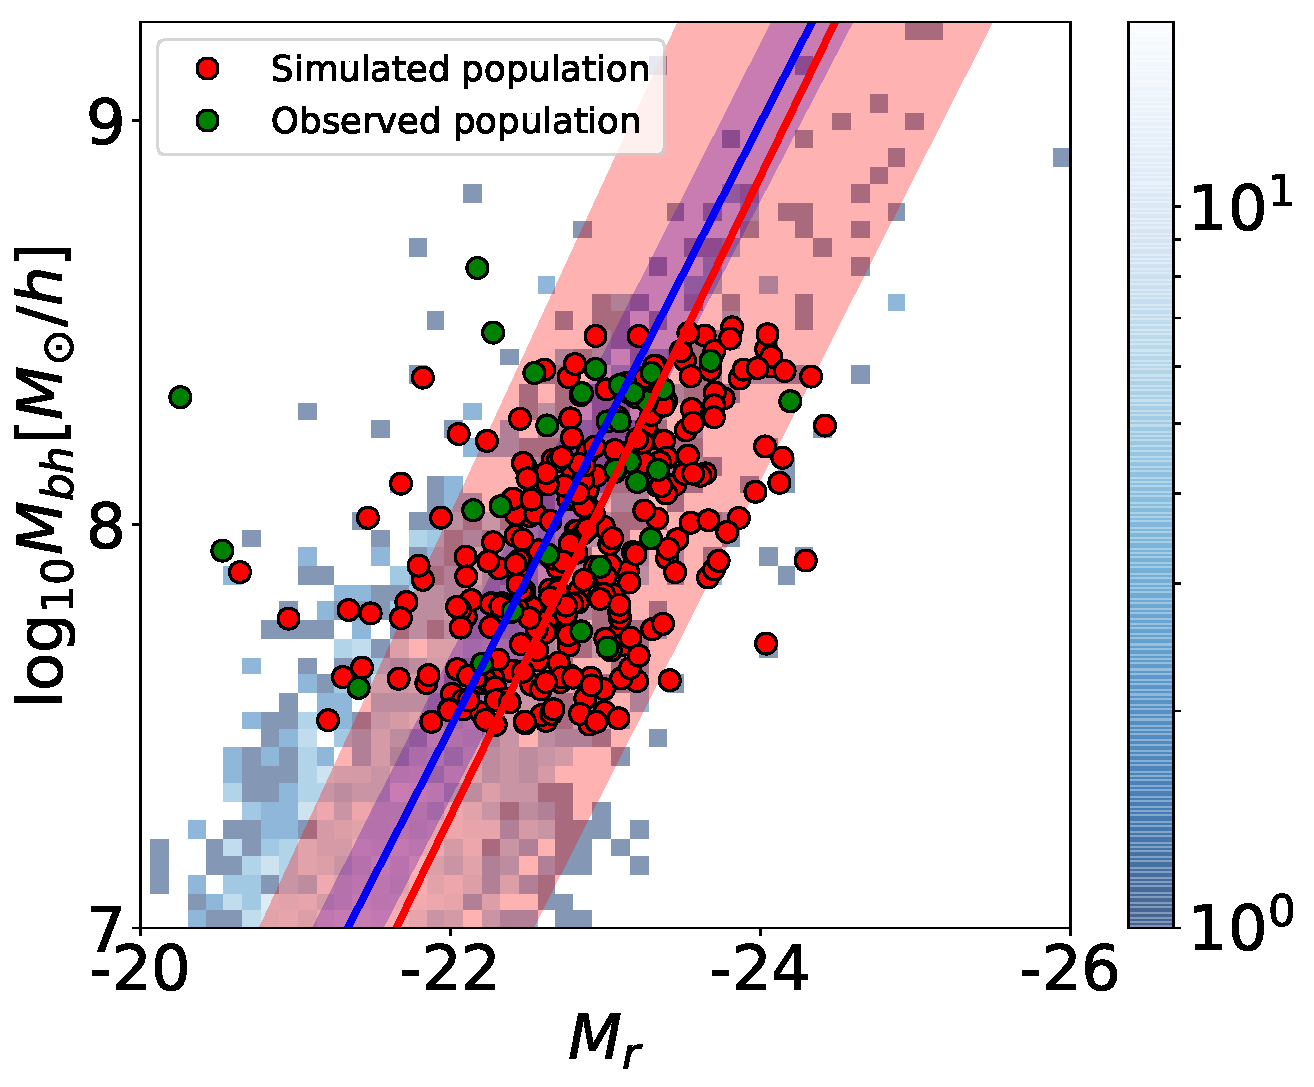
\includegraphics[trim = 0mm 0mm 61mm 0mm, clip, width=0.47\linewidth]{MBII_ML.pdf} &
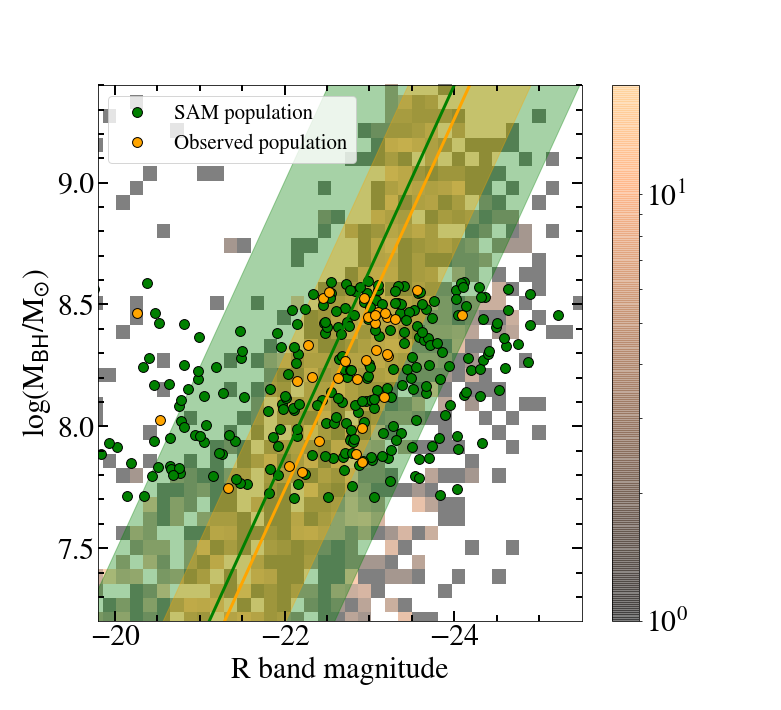
\includegraphics[trim = 0mm 0mm 61mm 0mm, clip, width=0.47\linewidth]{SAM_ML_consider_nois.pdf} \\
\end{tabular}
\caption{Same as the Figure~\ref{fig:MM_comp}, but for \mbh-\mr\ relation.}
\label{fig:ML_comp}
\end{figure*}


\begin{figure*}[t]%[!b]
\begin{tabular}{c c}
\includegraphics[width=0.45\linewidth]{comp_scatter_MM.pdf} &
\includegraphics[width=0.45\linewidth]{comp_scatter_ML.pdf} \\
\end{tabular}
\caption{The histogram of the scatter (i.e., residuals in the linear relation). The standard derivations for these distribution are $\sim0.3$~dex, $\sim0.3$~dex and $\sim0.7$~dex for observed sample, \mbii\ sample and \sam\ sample, respectively, for both \mbh-\mstar\ and \mbh-\mr\ relations.
}
\label{fig:offset_comp}
\end{figure*}

%%%%%%%%%%%%%%%%%%%%%%%%%%%%%%%%%%%%%%%%%%%%%%%%%%%%%

\section*{References}
\bibliography{references} 


\begin{addendum}
 \item[Acknowledgements] 
Based in part on observations made with the NASA/ESA Hubble Space Telescope, obtained at the Space Telescope Science Institute, which is operated by the Association of Universities for Research in Astronomy, Inc., under NASA contract NAS 5-26555. These observations are associated with programs \#15115. Support for this work was provided by NASA through grant number HST-GO-15115 from the Space Telescope Science Institute, which is operated by AURA, Inc., under NASA contract NAS 5-26555. The authors fully appreciate input from Simon Birrer, Matthew A. Malkan. XD and TT acknowledge support by the Packard Foundation through a Packard Research fellowship to TT. JS is supported by JSPS KAKENHI Grant Number JP18H01251 and the World Premier International Research Center Initiative (WPI), MEXT, Japan. TDM acknowledges funding from NSF ACI-1614853,  NSF AST-1616168 NASA ATP 80NSSC18K101 and NASA ATP 17-0123. We acknowledge support from INAF under PRIN SKA/ CTA FORECaST and PRIN SKA-CTA-INAF ASTRI/CTA Data Challenge. 

%
\item[Author Contributions] X.D. carried out the \hst\ data analysis, led the comparison to the simulating models and was the principal author of the paper. T.T. and J.S. designed the \hst\ project, selected the AGN sample, and wrote parts of the paper. A.B. and T.D. ran the \mbii\ simulation and provide the  \mbii\ data. N.M. ran the \sam\ model and provide and the \sam\ data. X.D, T.T, J.S., A.B., T.D., and N.M. interpreted the result.

\end{addendum}

%%%%%%%%%%%%%%%%%%%%%%%%%%%%%%%%%%%%%%%%%%%%%%%%%%%%%%%%%%%%%%%%%%%%%%%%%%%%%%%
\section*{Additional information}
%\textbf{Code availability.} The \lenstronomy, which is used to decompose the AGN image  
%The data reduction package used to process the \sam\ data is available at http://ascl.net/1407.006, and makes use of 2dfdr: http://www.aao.gov.au/science/software/2dfdr. To derive the stellar kinematic parameters and the lick absorption line strengths, we use the publicly available penalised pixel-fitting (pPXF) code from M. Capppellari: {http://www-astro.physics.ox.ac.uk/~mxc/software/\#ppxf}. For the adaptive LOESS smoothing, we use the code from M. Cappellari obtained from: http://www-astro.physics.ox.ac.uk/~mxc/software/\#loess

\textbf{Data availability.} All the inference of the AGN properties are presented in the companion paper.
%All reduced data-cubes in the GAMA fields used in this Letter are available on: http://datacentral.aao.gov.au/asvo/surveys/sami/, as part of the first SAMI Galaxy Survey data release. Stellar kinematic data products will become available in the second SAMI Galaxy Survey data release. 

\textbf{Correspondence and requests for materials} should be addressed to X.D.~(email:dxh@astro.ucla.edu).

%%%%%%%%%%%%%%%%%%%%%%%%%%%%%%%%%%%%%%%%%%%%%%%%%%%%%%%%%%%%%%%%%%%%%%%%%%%%%%%


%\clearpage
%\newpage
%\onecolumn
%\begin{center}
%{\bf \Large \uppercase{Supplementary information} }
%\end{center}
%
%\setcounter{figure}{0}
%\vspace{2cm}
%
%\begin{figure}[!h]
%\begin{center}
%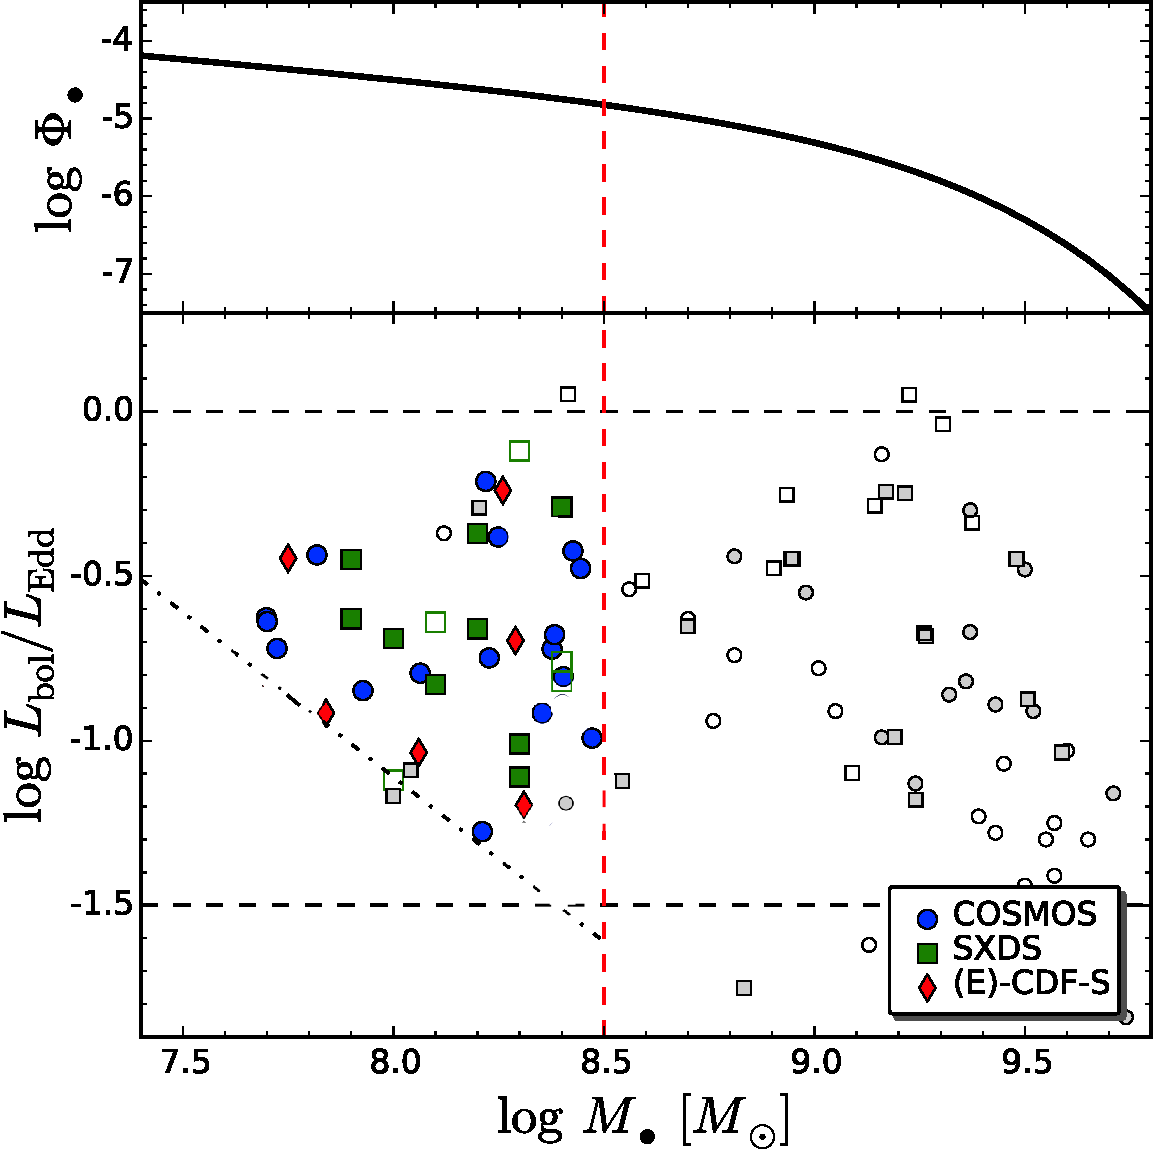
\includegraphics[width=0.8\linewidth]{hst_sample_bhmf.pdf}
%\caption{
%The selection function of our observation data. Eddington ratios (LBol/LEdd) and BH masses (bottom panel) of our sample (in color) that fall well-below the knee of the BH mass function at z = 1.5 (top panel; Schulze et al. 2015). Dashed lines (vertical and horizontal) denote our selection window with the slanted line only shown to approximately illustrate the effect of a luminosity limit, inherent in the parent catalogs. For reference, we indicate the high-z luminous SDSS QSO samples (grey squares - Peng et al. 2006; grey circles - Decarli et al. 2010) with all falling above our chosen upper mass limit.
%}
%\label{fig:support}
%\end{center}
%\end{figure}

\end{document}
